Constructions for a few basic Triangle Centers appear in Figure~\ref{fig:constructions}.

\begin{figure}
    \centering
    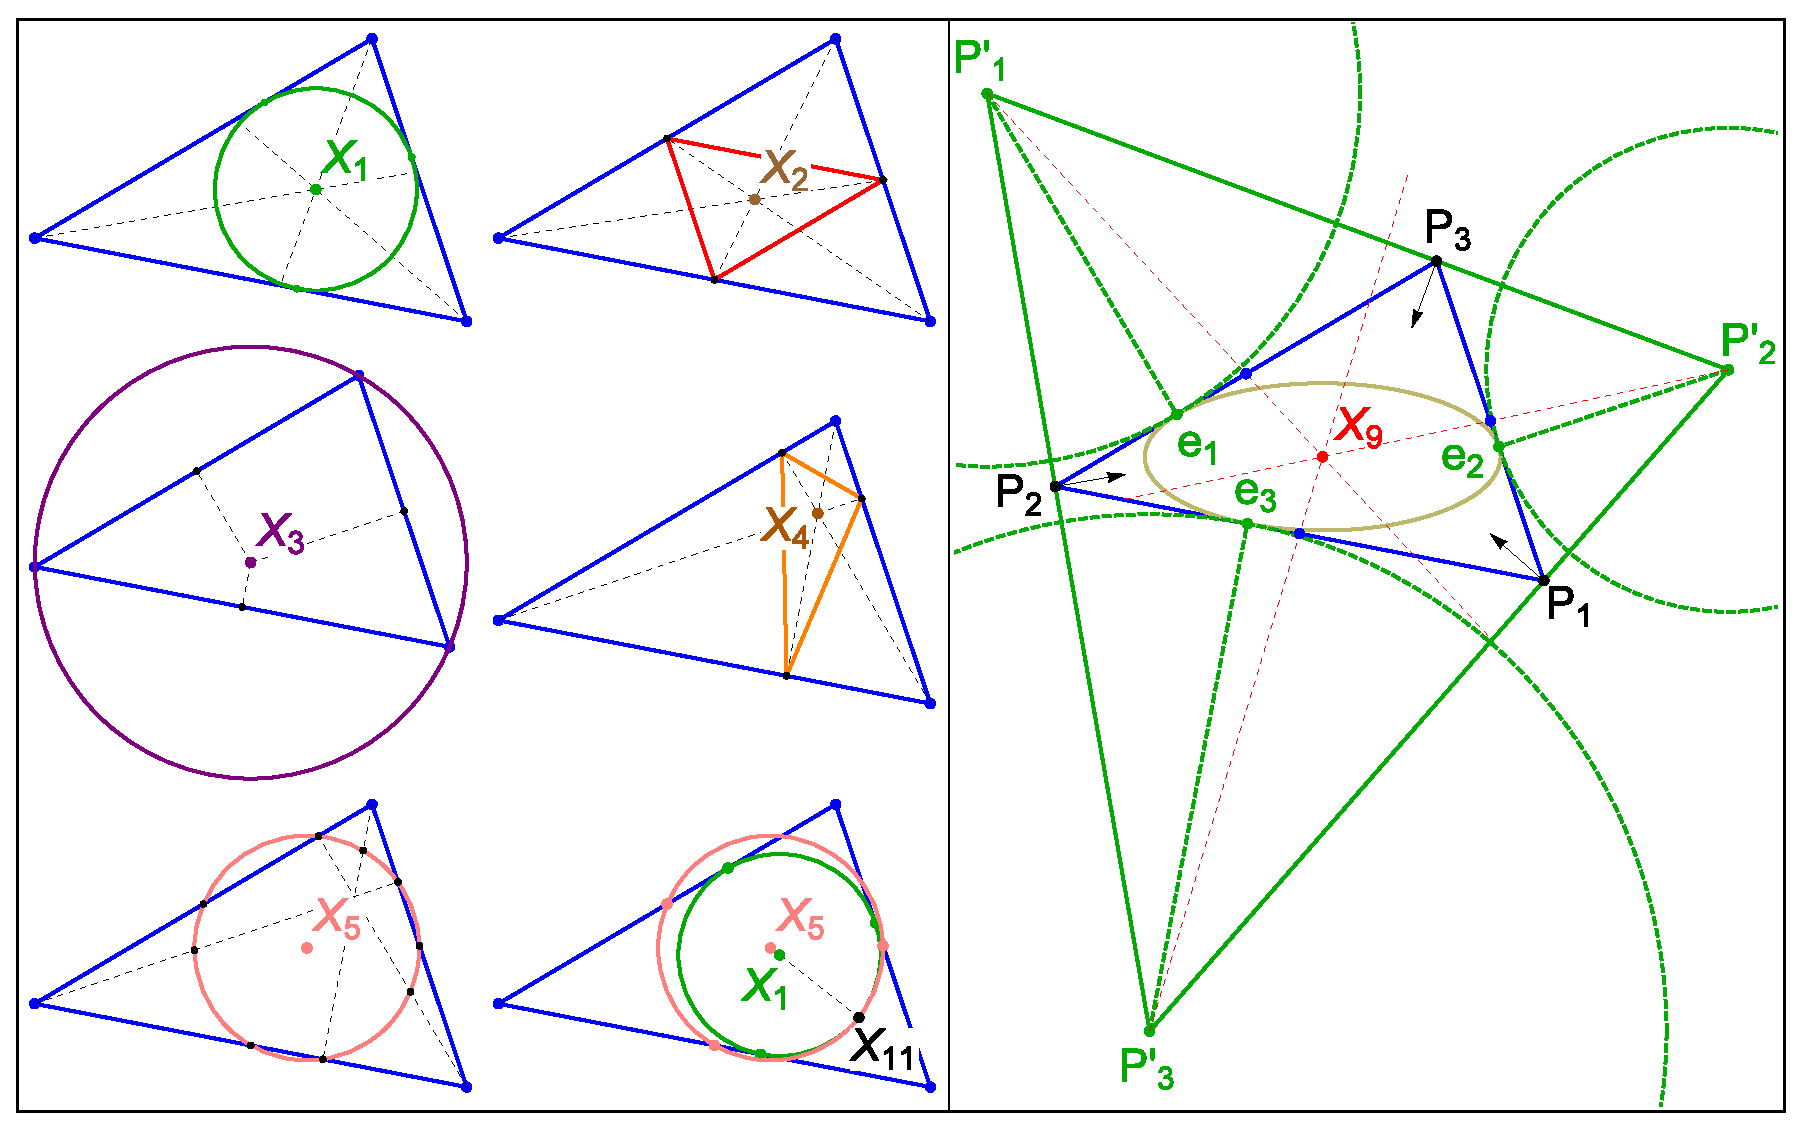
\includegraphics[width=\textwidth]{1010_pics_constr.eps}
    \caption{The construction of Basic Triangle Centers $X_i$, as listed in \cite{etc}. \textbf{Left}: The Incenter $X_1$ is the intersection of angular bisectors, and center of the Incircle (green), a circle tangent to the sides at three {\em Intouchpoints} (green dots), its radius is the {\em Inradius} $r$. The Barycenter $X_2$ is where lines drawn from the vertices to opposite sides' midpoints meet. Side midpoints define the {\em Medial Triangle} (red). The Circumcenter $X_3$ is the intersection of perpendicular bisectors, the center of the {\em Circumcircle} (purple) whose radius is the {\em Circumradius} $R$. The Orthocenter $X_4$ is where altitudes concur. Their feet define the {\em Orthic Triangle} (orange). $X_5$ is the center of the 9-Point (or Euler) Circle (pink): it passes through each side's midpoint, altitude feet, and Euler Points \cite{mw}. The Feuerbach Point $X_{11}$ is the single point of contact between the Incircle and the 9-Point Circle. \textbf{Right}: given a reference triangle $P_1P_2P_3$ (blue), the {\em Excenters} $P_1'P_2'P_3'$ are pairwise intersections of lines through the $P_i$ and perpendicular to the bisectors. This triad defines the {\em Excentral Triangle} (green). The {\em Excircles} (dashed green) are centered on the Excenters and are touch each side at an {\em Extouch Point} $e_i,i=1,2,3$. Lines drawn from each Excenter through sides' midpoints (dashed red) concur at the {\em Mittenpunkt} $X_9$. Also shown (brown) is the triangle's {\em Mandart Inellipse}, internally tangent to each side at the $e_i$, and centered on $X_9$. This is identical to the $N=3$ Caustic.}
    \label{fig:constructions}
\end{figure}

Any point on the plane of a triangle $T=P_1P_2P_3$ can be defined by specifying a triple of {\em Trilinear Coordinates} $x:y:z$ which are proportional to the signed distances from $P$ to each side, which makes them invariant under similarity, and reflection transformations.

A {\em Triangle Center} (with respect to a triangle $T={P_1}{P_2}{P_3}$) is defined by Trilinear Coordinates obtained by thrice applying a {\em Triangle Center Function} $h$ to the sidelengths as follows:
 
\begin{equation}
\label{eqn:ftrilins}
    x:y:z {\iff} h(s_1,s_2,s_3):h(s_2,s_3,s_1):h(s_3,s_1,s_2)
\end{equation}

$h$ must (i) be {\em bi-symmetric}, i.e., $h(s_1,s_2,s_3)=h(s_1,s_3,s_2)$, and (ii) homogeneous, $h(t s_1, t s_2, t s_3)=t^n h(s_1,s_2,s_3)$ for some $n$ \cite{kimberling1993_rocky}. Trilinears for nearly 40k Triangle centers are available in \cite{etc}. Trilinears can be converted to Cartesians using \cite{mw}:
  
\begin{equation}
\label{eqn:trilin-cartesian}
X_i|_{\text{cartesian}}=\frac{s_1 x P_1 + s_2 y P_2 + s_3 z P_3}{D}
\end{equation}

Where and $D={s_1}x+{s_2}y+{s_3}z$.
